\documentclass[a4paper,11pt]{article}

\usepackage{etoolbox}
\usepackage{fancyvrb}
\usepackage[T1]{fontenc}
\usepackage{graphicx}
\usepackage{import}
\usepackage{listings}
\usepackage{minted}
\usepackage{url}

\usepackage[
	% Prevent hyperlinks from getting an ugly border
    hidelinks,
    % Set proper PDF metadata
    pdftex,
    pdfauthor={Dennis Fischer},
    pdftitle={TBD},
    pdfsubject={TBD},
    pdfkeywords={TBD}
]{hyperref}

\usepackage{sections/_meta/tumlogo}

% Don't display "References" when rendering the bibliography
\patchcmd{\thebibliography}{\section*{\refname}}{}{}{}

% Use appropriate font size for line numbers in listings
\renewcommand{\theFancyVerbLine}{{\small\arabic{FancyVerbLine}}}

\lstset{basicstyle=\ttfamily}
\newcommand{\code}[1]{\texttt{#1}}

\setlength{\footnotesep}{0.4cm}
\setlength{\skip\footins}{0.5cm}

\def\doctype{Bachelor's Thesis in Informatics}
\def\title{TBD}
\def\germantitle{TBD}
\def\author{Dennis Fischer}
\def\date{Februar 15, 2016}

\begin{document}

\thispagestyle{empty}

\def\bcorcor{0.15cm}
\addtolength{\hoffset}{\bcorcor}

\thispagestyle{empty}

\vspace{4cm}

\begin{center}
  \oTUM{4cm}
  
  \vspace{5mm}
  
  \huge DEPARTMENT OF INFORMATICS\\
  
  \vspace{0.5cm}
  
  \large TECHNISCHE UNIVERSIT{\"A}T M{\"U}NCHEN\\
  
  \vspace{1mm}
\end{center}

\vspace{15mm}

\begin{center}
  {\Large \doctype}

  \vspace{20mm}

  \setlength\lineskip{8pt}
  {\LARGE \bf \title}\\%[3ex]

  \vspace{15mm}

  {\LARGE \author}

  \vspace{10mm}

  \begin{figure}[h!]
    \centering
    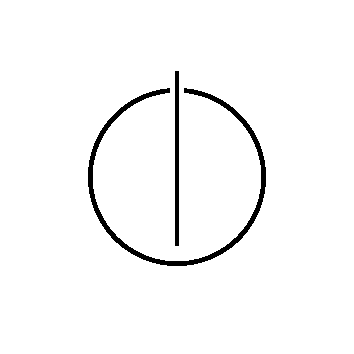
\includegraphics[width=4cm]{sections/_meta/informat.png}
  \end{figure}
\end{center}

\thispagestyle{empty}

\def\bcorcor{0.15cm}
\addtolength{\hoffset}{\bcorcor}

\thispagestyle{empty}

\vspace{4cm}

\begin{center}
  \oTUM{4cm}
  
  \vspace{5mm}
  
  \huge DEPARTMENT OF INFORMATICS\\
  
  \vspace{0.5cm}
  
  \large TECHNISCHE UNIVERSIT{\"A}T M{\"U}NCHEN\\
  
  \vspace{1mm}
\end{center}

\vspace{15mm}

\begin{center}
  {\Large \doctype}

  \vspace{20mm}

  \setlength\lineskip{8pt}
  {\LARGE \bf \title}\\%[3ex]

  \vspace{10mm}

  {\LARGE \germantitle}
\end{center}

\vfill

\renewcommand{\arraystretch}{0.7}

\begin{center}
\begin{tabular}{l@{\hskip 1cm}l}
  {\Large \bf Author:} & {\Large Dennis~Fischer} \\\\
  {\Large \bf Supervisor:} & {\Large Prof.~Dr.~Alexander~Pretschner} \\\\
  {\Large \bf Advisor:} & {\Large M.Sc.~Sebastian Banescu} \\\\
  {\Large \bf Submission date:} & {\Large 15.~Februar~2016}
\end{tabular}
\end{center}

\thispagestyle{empty}

\vspace*{\fill}
\begin{flushright}
\noindent \textit{I confirm that this bachelor's thesis is my own work \\ and I have documented all sources and material used.\\[\baselineskip]}
M{\"u}nchen, 15. Februar 2016 \\[3.5\baselineskip]
\underline{\hspace{6.5cm}}
\end{flushright}


\newpage
\thispagestyle{empty}
\null

%\newpage
\thispagestyle{empty}
\section*{Abstract}

TBD

\newpage
\pagestyle{empty}
\tableofcontents

\newpage
\pagestyle{plain}
\setcounter{page}{1}

%PUT Content here!

\section{References}
\bibliography{references}
\bibliographystyle{plain}

%PUT Appendix here!

\end{document}
